% Se pre-carga la información del estudiante sólo para poder emplear el macro de
% selección de versión (digital o impresa)
% =============================================================================
% El estudiante debe llenar sus datos en esta sección para que la plantilla los 
% auto-importe y genere automáticamente las páginas de portada y de firmas 
% autorizadas.
% =============================================================================
% Datos del estudiante:
% -----------------------------------------------------------------------------
% Nombre completo
\def \nombreestudiante {Albert Vandercam Hart}
% Carné
\def \uvgcarne {22688}
% Facultad
\def \uvgfacultad {Ingeniería}
% Carrera
\def \uvgcarrera {Ingeniería Mecatrónica}


% Datos del trabajo:
% -----------------------------------------------------------------------------
% Título completo
\def \titulotesis {Control de drones basado en gestos mediante captura de movimiento en el ecosistema Robotat}
% Año de entrega
\def \anoentrega {2026}
% Asesor
\def \nombreasesor {PhD. Luis Alberto Rivera Estrada}
% Modalidad del trabajo de graduación 
% Tesis, si defienden ante terna
% Trabajo Profesional, de otra manera
% Comente la siguiente línea si su trabajo corresponde a modalidad de Trabajo Profesional (se deja Tesis por defecto)
%\def \modgraduacion {Tesis}

% Año de aprobación
\def \anoaprobacion {2026}
% Mes de aprobación
\def \mesaprobacion {noviembre }
% Día de aprobación
\def \diaaprobacion {24 }

% Datos para modalidad Tesis:
% -----------------------------------------------------------------------------
\ifdefined\modgraduacion 
% Datos del tribunal examinador:
% Nombre del primer examinador
\def \nombreprimerex {Mgtr. Kurt Kellner}
% Nombre del segundo examinador
\def \nombresegundoex {MBA. Pedro Castillo}

% Datos para modalidad Trabajo Profesional:
% -----------------------------------------------------------------------------
\else
\def \modgraduacion {Trabajo Profesional}
% Nombre del director de la carrera
\def \nombredirector {MSc. Carlos Esquit}
\def \twosignatures
\fi

% Capítulos pre-definidos
% -----------------------------------------------------------------------------
% Comentar las líneas de las secciones que desean omitirse, por defecto se 
% se incluyen todas.
\def \CAPprefacio {Prefacio}
\def \CAPantecedentes {Antecedentes}
\def \CAPanexos {Anexos}
\def \CAPglosario {Glosario}

% Sólo puede activarse UNA de las siguientes tres opciones, dependiendo de lo que se requiera (revisar la guía de redacción de trabajos de graduación).
\def \CAPhipotesis {Hipótesis}
%\def \CAPdefinicion {Definición del problema}
%\def \CAPalcance {Alcance}


% Formato y estilo de la plantilla
% -----------------------------------------------------------------------------
% Referencias: Puede des-comentar la siguiente línea para utilizar el formato de referencias APA
%def \usarAPA {Usar formato APA}

% Hoja de firmas: Puede des-comentarse la siguiente línea si, en lugar de colocar la hoja de firmas en el archivo hoja_firmas.pdf, desea generarse la misma empleando la información de los asesores y miembros de la terna, para ser firmada dentro del documento.
\def \GENfirmas {Hoja de firmas}

% Portada: Puede cambiarse la imagen en la portada al cambiar el nombre del 
% archivo siguiente. NOTA: la imagen debe tener la suficiente resolución (1920x768, o más grande pero con una relación 2.5:1) para cubrir el área designada. Por defecto se coloca la imagen del CIT.
\def \imagenportada {plantilla/portadacit-real.png}








\documentclass[11pt, letterpaper]{report}

% Eliminar la opción de twoside y openright si se desea generar la versión
% digital del documento en lugar de la versión impresa
%\documentclass[11pt, letterpaper, twoside, openright]{report}
\usepackage[spanish, es-nodecimaldot, es-noquoting]{babel}
% cambiar a spanish, mexico si se quiere emplear tabla en lugar de cuadro
\selectlanguage{spanish}
\usepackage[utf8]{inputenc}
\usepackage[T1]{fontenc}

\title{Plantilla para Trabajos de Graduación 2025v5}
\author{MSc. Miguel Zea}
\date{\today}

% Información del estudiante en el archivo datos_estudiante.tex
% =============================================================================
% El estudiante debe llenar sus datos en esta sección para que la plantilla los 
% auto-importe y genere automáticamente las páginas de portada y de firmas 
% autorizadas.
% =============================================================================
% Datos del estudiante:
% -----------------------------------------------------------------------------
% Nombre completo
\def \nombreestudiante {Albert Vandercam Hart}
% Carné
\def \uvgcarne {22688}
% Facultad
\def \uvgfacultad {Ingeniería}
% Carrera
\def \uvgcarrera {Ingeniería Mecatrónica}


% Datos del trabajo:
% -----------------------------------------------------------------------------
% Título completo
\def \titulotesis {Control de drones basado en gestos mediante captura de movimiento en el ecosistema Robotat}
% Año de entrega
\def \anoentrega {2026}
% Asesor
\def \nombreasesor {PhD. Luis Alberto Rivera Estrada}
% Modalidad del trabajo de graduación 
% Tesis, si defienden ante terna
% Trabajo Profesional, de otra manera
% Comente la siguiente línea si su trabajo corresponde a modalidad de Trabajo Profesional (se deja Tesis por defecto)
%\def \modgraduacion {Tesis}

% Año de aprobación
\def \anoaprobacion {2026}
% Mes de aprobación
\def \mesaprobacion {noviembre }
% Día de aprobación
\def \diaaprobacion {24 }

% Datos para modalidad Tesis:
% -----------------------------------------------------------------------------
\ifdefined\modgraduacion 
% Datos del tribunal examinador:
% Nombre del primer examinador
\def \nombreprimerex {Mgtr. Kurt Kellner}
% Nombre del segundo examinador
\def \nombresegundoex {MBA. Pedro Castillo}

% Datos para modalidad Trabajo Profesional:
% -----------------------------------------------------------------------------
\else
\def \modgraduacion {Trabajo Profesional}
% Nombre del director de la carrera
\def \nombredirector {MSc. Carlos Esquit}
\def \twosignatures
\fi

% Capítulos pre-definidos
% -----------------------------------------------------------------------------
% Comentar las líneas de las secciones que desean omitirse, por defecto se 
% se incluyen todas.
\def \CAPprefacio {Prefacio}
\def \CAPantecedentes {Antecedentes}
\def \CAPanexos {Anexos}
\def \CAPglosario {Glosario}

% Sólo puede activarse UNA de las siguientes tres opciones, dependiendo de lo que se requiera (revisar la guía de redacción de trabajos de graduación).
\def \CAPhipotesis {Hipótesis}
%\def \CAPdefinicion {Definición del problema}
%\def \CAPalcance {Alcance}


% Formato y estilo de la plantilla
% -----------------------------------------------------------------------------
% Referencias: Puede des-comentar la siguiente línea para utilizar el formato de referencias APA
%def \usarAPA {Usar formato APA}

% Hoja de firmas: Puede des-comentarse la siguiente línea si, en lugar de colocar la hoja de firmas en el archivo hoja_firmas.pdf, desea generarse la misma empleando la información de los asesores y miembros de la terna, para ser firmada dentro del documento.
\def \GENfirmas {Hoja de firmas}

% Portada: Puede cambiarse la imagen en la portada al cambiar el nombre del 
% archivo siguiente. NOTA: la imagen debe tener la suficiente resolución (1920x768, o más grande pero con una relación 2.5:1) para cubrir el área designada. Por defecto se coloca la imagen del CIT.
\def \imagenportada {plantilla/portadacit-real.png}







\input{1-opciones_adicionales}

% ============================================================================
% DEFINICIÓN DE PAQUETES
% ============================================================================
\usepackage{xcolor}
\usepackage{amsfonts}
\usepackage{amsmath}
\usepackage{amssymb}
\usepackage{amsthm}
\usepackage{amsfonts}
\usepackage{mathtools}
\usepackage{graphicx}
\usepackage{xfrac}
\usepackage{float}
\usepackage{mathtools}
\usepackage[hypertexnames=false, hidelinks]{hyperref}
% \usepackage{bookmark}
\usepackage[font=small, labelsep=period, labelfont=bf]{caption}
\usepackage{subcaption}
\usepackage{csquotes}
\usepackage{xpatch}
\usepackage{emptypage}
\usepackage{hyphenat}
\usepackage{fancyhdr}
\usepackage{pdfpages}
\usepackage{verbatim}

\ifdefined\usarAPA 
    \usepackage[backend=biber, style=apa]{biblatex}
\else
    \usepackage[backend=biber, style=ieee, maxnames=99]{biblatex} %maxnames=99
\fi
\addbibresource{m-bibliografia.bib}

\usepackage{chngcntr}
\captionsetup{justification=raggedright, singlelinecheck=false, format=hang}

\ifdefined\CAPglosario
	%\usepackage[toc]{glossaries}
	\usepackage[numberedsection]{glossaries}
	\makeglossaries
    \input{o-glosario}
\fi

% ============================================================================
% MÁRGENES Y FORMATO GENERALES
% ============================================================================
\usepackage[top=1in, left=1.5in, right=1in, bottom=1in]{geometry}
%Options: Sonny, Lenny, Glenn, Conny, Rejne, Bjarne, Bjornstrup
\usepackage[Sonny]{fncychap}

% Penalizaciones para evitar "widows" y "orphans", es decir, dejar sólo una línea de inicio o final de un párrafo en una página distinta al resto del párrafo
\clubpenalty=10000
\widowpenalty=10000
\displaywidowpenalty=10000

% ============================================================================
% DEFINICIONES DE LA PLANTILLA
% ============================================================================
\graphicspath{ {figuras/} }
\definecolor{uvg-green}{RGB}{17,71,52}
\newcommand{\defaultparformat}[1]{
	{\setlength{\parskip}{2ex}
     \input{#1}}
}

\counterwithout{figure}{chapter}
\counterwithout{table}{chapter}
\counterwithout{equation}{chapter}

\newcommand{\blankpage}{
\newpage
\thispagestyle{empty}
\mbox{}
\newpage
}

\newcommand{\note}[1]{\vspace*{0.5em} \caption*{Nota. #1}}
\newcommand{\palabrasclave}[1]{\textbf{Palabras clave: } #1.}
\newcommand{\keywords}[1]{\textbf{Keywords: } #1.}

\setcounter{tocdepth}{1}

% Párrafo: Puede comentar la siguiente línea si desea emplear un formato de 
% párrafo distinto al establecido por defecto
\def \parpordefecto {Formato de párrafo por defecto}

% --- LoF: show "Figura/Figure <n>." before caption text ---
\makeatletter
\renewcommand*\l@figure[2]{%
  \begingroup
    % Use \figurename so it follows babel ("Figura" in spanish, "Figure" in english)
    \def\numberline##1{\figurename~##1.\hspace{0.6em}}%
    % indent=1.5em is the default; numwidth widened to fit "Figura 123."
    \@dottedtocline{1}{1.5em}{5.0em}{#1}{#2}%
  \endgroup
}
\makeatother

% --- LoF: do the same for Tables/Cuadros  ---
\makeatletter
\renewcommand*\l@table[2]{%
  \begingroup
    \def\numberline##1{\tablename~##1.\hspace{0.6em}}%
    \@dottedtocline{1}{1.5em}{5.0em}{#1}{#2}%
  \endgroup
}
\makeatother
% ============================================================================

% Comandos definidos por el usuario en el archivo comandos_usuario.tex
\input{2-paquetes_y_comandos_usuario}

% ============================================================================
% CUERPO DEL TRABAJO
% ============================================================================
\pagestyle{headings}
\begin{document}

% Se define la carpeta de imágenes
\graphicspath{{figuras/}}

% ============================================================================
% PORTADA
% ============================================================================
\ifdefined\CAPportada
    \cleardoublepage\phantomsection
    % \pdfbookmark{Portada}{toc}
	\newgeometry{left=3cm, bottom=0in, top=1in, right=3cm}
	\pagecolor{uvg-green}
	\thispagestyle{empty}

	\color{white}
	\noindent \hrulefill \par
	\vspace{0.1in}
	\noindent \Huge \nohyphens{\titulotesis} \par
	\noindent \hrulefill \par
	\noindent
	\LARGE \nombreestudiante

    \begin{figure}[b!]
    	\makebox[\textwidth] {
            \centering
            \includegraphics[height=4.5in]{\imagenportada}
    	}
        \centering
        
\includegraphics[height=1in]{plantilla/logoUVGblanco.png}  
	\end{figure}

	\restoregeometry
\fi

% ============================================================================
% PRIMERAS PÁGINAS (Carátulas más hojas de guarda)
% ============================================================================
\ifdefined\CAPcaratula
    \pagecolor{white}
	\color{black}
    \blankpage
    
    \newpage
    \cleardoublepage\phantomsection
    % \pdfbookmark{Carátula}{toc}
	\setcounter{page}{1}
	\pagenumbering{roman}
	\thispagestyle{empty}
	\begin{center}
		\LARGE UNIVERSIDAD DEL VALLE DE GUATEMALA\\
		\LARGE Facultad de \uvgfacultad \\[0.75cm]
	\end{center}
	\begin{figure}[h]
		\begin{center}
		
\includegraphics[height=5.5 cm]{plantilla/escudoUVGcolores.eps}
		\vspace{0.5in}
		\end{center}
	\end{figure}
	\begin{center}
		\Large \textbf{\nohyphens{\titulotesis}} \\
		%\LARGE \textbf{\titulotesis} \\
		\vfill
		\Large \nohyphens{Trabajo de graduación en modalidad de \modgraduacion, presentado por \nombreestudiante \ para optar al grado académico de Licenciado en \uvgcarrera} \\
		\vfill
		\large Guatemala, \\
		\vspace{1em}
		\anoentrega
	\end{center}
    
\fi

% ============================================================================
% HOJA DE FIRMAS
% ============================================================================
% Ya sea se genera la hoja de firmas
\ifdefined\GENfirmas
	\ifdefined \twosignatures
        \newpage
    	\cleardoublepage\phantomsection
    	\thispagestyle{empty}
    	\vspace*{2.25in}
    	\large Vo.Bo.:\\[1cm]
    	\begin{center}
    		(f) \rule[1pt]{4 in}{1pt}\\
    		\nombreasesor \\[1in]
    		(f) \rule[1pt]{4 in}{1pt}\\
    		\nombredirector
    	\end{center}
    	\vspace{2.25in}

        Fecha de aprobación: Guatemala, \diaaprobacion de \mesaprobacion de \anoaprobacion.
    	\normalsize

    \else
        \newpage
    	\cleardoublepage\phantomsection
    	\thispagestyle{empty}
    	\vspace*{0.5in}
    	\large Vo.Bo.:\\[1cm]
    	\begin{center}
    		(f) \rule[1pt]{4 in}{1pt}\\
    		\nombreasesor
    	\end{center}
    	\vspace{1in}
    
    	Tribunal Examinador:\\[1cm]
    	\begin{center}
    		(f) \rule[1pt]{4 in}{1pt}\\
    		\nombreasesor \\[1in]
    		(f) \rule[1pt]{4 in}{1pt}\\
    		\nombreprimerex \\[1in]
    		(f) \rule[1pt]{4 in}{1pt}\\
    		\nombresegundoex
    	\end{center}
    	\vspace{1in}
    
        Fecha de aprobación: Guatemala, \diaaprobacion de \mesaprobacion de \anoaprobacion.
    	\normalsize
    \fi
    
% O se adjunta la hoja firmada, que debe estar contenida en el documento hoja_firmas.pdf
\else
    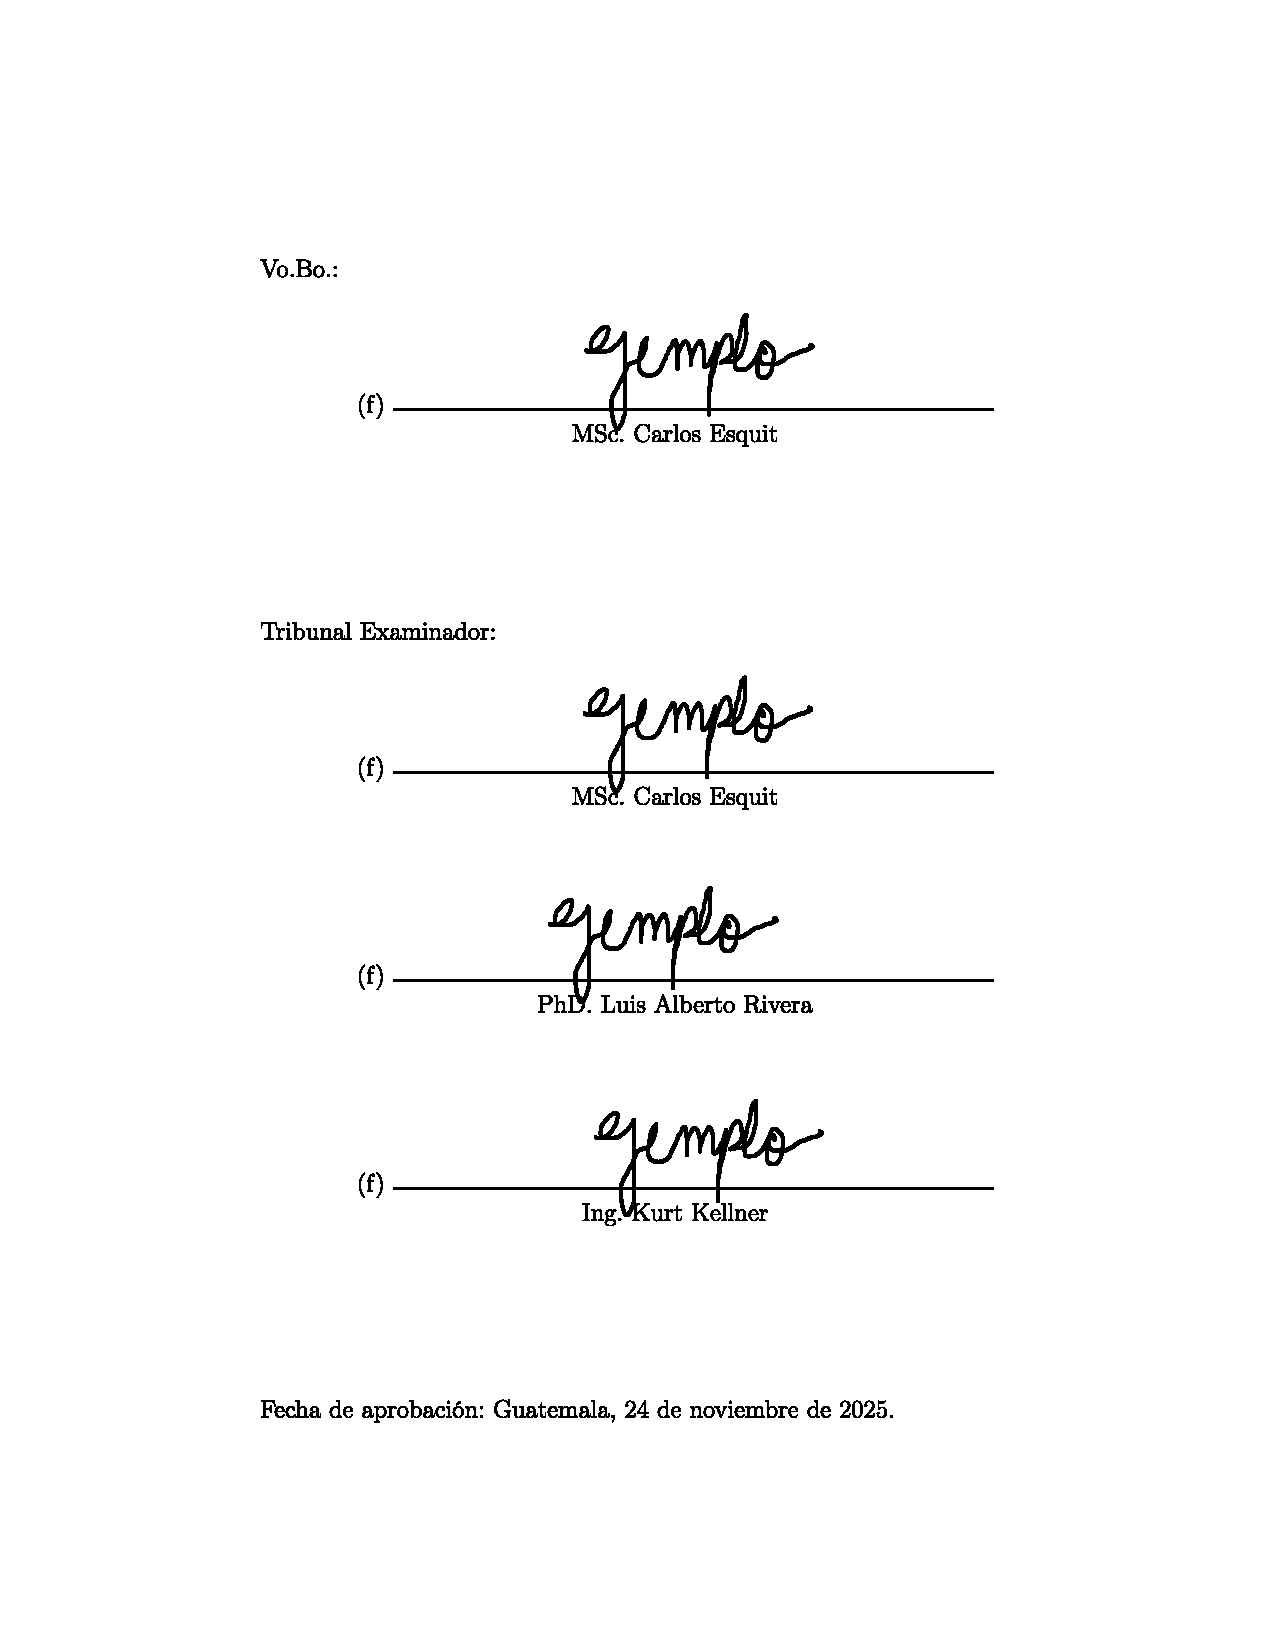
\includepdf[pages={1}]{hoja_firmas.pdf}
    \normalsize
\fi

% Comentar para formato estilo libro en la numeración de páginas (NO 
% compatible con la guía UVG 2019)
\pagestyle{plain}
% ============================================================================
% CONTENIDO DEL TRABAJO
% ============================================================================
% PREFACIO
% ----------------------------------------------------------------------------
\ifdefined\CAPprefacio
	\newpage
	\cleardoublepage\phantomsection
    \setcounter{page}{1}
    \chapter*{Prefacio}
    \ifdefined\parpordefecto
    	\defaultparformat{a-prefacio}
    \else
    	Bienvenido a la plantilla de \LaTeX para trabajos de graduación de la Universidad del Valle de Guatemala. El objetivo principal de la misma es facilitar la redacción del contenido del trabajo, evitando los posibles problemas que puedan surgir con el formato. En cada sección se incluye una breve descripción sobre qué debe contener la misma (esto corresponde a la información contenida en la guía oficial de la universidad para la redacción de trabajos de graduación), y más adelante se explicará el uso de la plantilla como tal.

\noindent\rule{\linewidth}{0.4pt}

El prefacio es opcional y se coloca antes del índice general. Es la primera que lleva numeración de página con números romanos. Aquí se da las gracias a colaboradores, familia, amigos, etc.; por lo tanto, no debe agregarse un capítulo de agradecimientos. 

En este capítulo, se agradece a las personas o entidades que apoyaron al trabajo; \textbf{no es la introducción}.
    \fi
    \addcontentsline{toc}{chapter}{Prefacio}
\fi

% ÍNDICE GENERAL
% ----------------------------------------------------------------------------
\ifdefined\CAPindice
	\newpage
    \cleardoublepage\phantomsection
	\renewcommand{\contentsname}{Índice general}
    %\phantomsection
    \pdfbookmark{\contentsname}{toc}
    %\pdfbookmark{Índice}{toc}
	\tableofcontents
\fi

% ÍNDICE DE FIGURAS
% ----------------------------------------------------------------------------
\ifdefined\CAPfiguras
	\newpage
    \cleardoublepage\phantomsection
	\renewcommand{\listfigurename}{Índice de figuras}
	\listoffigures
	\addcontentsline{toc}{chapter}{Índice de figuras}
\fi

% ÍNDICE DE CUADROS
% ----------------------------------------------------------------------------
\ifdefined\CAPcuadros
	\newpage
    \cleardoublepage\phantomsection
	\renewcommand{\listtablename}{Índice de cuadros}
	\listoftables
	\addcontentsline{toc}{chapter}{Índice de cuadros}
\fi

% RESUMEN
% ----------------------------------------------------------------------------
\ifdefined\CAPresumen
	\newpage
    \cleardoublepage\phantomsection
	\chapter*{Resumen}
	\ifdefined\parpordefecto
		\defaultparformat{b-resumen}
	\else
		Todo trabajo de graduación requiere un resumen, pues sirve para que el lector adquiera una visión completa de la materia tratada. Se sugiere colocarlo antes de la introducción porque, en su paso por el índice, el lector ya habrá obtenido una idea general del trabajo, por lo que decidirá si sigue leyendo o no. El resumen aborda una visión general del problema, los objetivos, la metodología y los resultados, sin explicar nada.  

Al final, se incluye una lista de palabras clave (tres mínimo; cinco máximo). Se escriben con minúsculas, separadas por coma. Pueden ser individuales o compuestas, por ejemplo: «educación a distancia», «medicina alternativa», «legislación laboral». Para elegirlas, puede apoyarse de herramientas de IA que ayuden a identificar cuáles serían las mejores palabras clave para motores de búsqueda académicos.

La extensión del resumen es de 250 palabras, por lo que debe ser conciso en la información que brinda.

\palabrasclave{Inteligencia artificial, STEM, ingeniería, \textit{keywords in English}}
	\fi
	\addcontentsline{toc}{chapter}{Resumen}
\fi

% ABSTRACT
% ----------------------------------------------------------------------------
\ifdefined\CAPabstract
	\newpage
    \cleardoublepage\phantomsection
	\chapter*{Abstract}
	\ifdefined\parpordefecto
		\defaultparformat{c-abstract}
	\else
		El \textit{abstract} es la traducción al inglés del resumen, incluyendo las palabras clave \textit{(keywords)}. Esto se hace para la difusión del conocimiento, ya que los trabajos de graduación desarrollan información importante y valiosa que debe estar disponible para todos.

\keywords{Artificial intelligence, STEM, engineering, keywords in English}
	\fi
	\addcontentsline{toc}{chapter}{Abstract}
\fi

% INTRODUCCIÓN
% ----------------------------------------------------------------------------
\ifdefined\CAPintroduccion
	\newpage
	\cleardoublepage
	\pagenumbering{arabic}
	\setcounter{page}{1}
	\chapter{Introducción}
	\ifdefined\parpordefecto
		\defaultparformat{d-introduccion}
	\else
		La introducción antecede al cuerpo del trabajo, pero se escribe de último. Constituye el primer capítulo y la página número uno. A diferencia del resumen, es más extenso, pues contextualiza y describe la composición del trabajo. Suele incluirse la siguiente información:

\begin{itemize}
    \item Campo de estudio.

    \item Finalidad del trabajo.

    \item Delimitación y definición del tema.

    \item Metodología y procedimientos, sin mayor detalle, ya que tienen su capítulo aparte.

    \item Conclusiones más importantes.
    
\end{itemize}

      

      

      

      

      
	\fi
\fi

% ANTECEDENTES
% ----------------------------------------------------------------------------
\ifdefined\CAPantecedentes
	\newpage
	\chapter{Antecedentes}
	\ifdefined\parpordefecto
    	\defaultparformat{e-antecedentes}
    \else
    	La Universidad del Valle de Guatemala se ha preocupado por el desarrollo de tecnología en esta área, particularmente empleando plataformas como el Crazyflie 2.1, con el objetivo de mejorar su eficiencia, seguridad y facilidad de uso. En 2025, Angela Figueroa \cite{figueroa2025desarrollo} y César Schwendener \cite{schwendener2025desarrollo}, estudiantes de la Universidad del Valle de Guatemala, estuvieron trabajando en la optimización de la infraestructura experimental y en herramientas de software para el control y evaluación del cuadricóptero Crazyflie 2.1. Sus resultados fueron satisfactorios, obteniendo una forma de controlar los drones utilizando \textit{Python} y reduciendo la latencia entre la computadora y el agente mediante mejoras en la comunicación. 

 

Debido a esta problemática, existen investigaciones relacionadas con el control de drones por medio de movimientos naturales, buscando una interacción más intuitiva. En 2016, Obaid et al. \cite{obaid2016would} realizaron un estudio centrado en el usuario para analizar cómo las personas podrían controlar drones mediante movimientos corporales. El objetivo fue definir un conjunto de acciones intuitivas para la navegación aérea. Más de 300 propuestas fueron recopiladas y analizadas, llegando a la conclusión de que existe un conjunto de comandos comunes en los cuales múltiples participantes coincidieron al realizar el mismo movimiento para representar acciones específicas como desplazamiento o rotación. Los resultados reflejaron que un  89\% de los gestos utilizados fueron dinámicos, a su vez el 45\% de las personas usan una mano para controlar un dron y el  42\% usaron ambas manos.

De manera similar,  se ha explorado la implementación física de estos sistemas de interacción corporal. En Suiza, Rognon et al. \cite{8304759} desarrollaron el exoesqueleto \textit{FlyJacket} para el control inmersivo de drones. Esta investigación tenía como objetivo hacer más accesible el control de drones mediante inclinaciones del torso, proporcionando una experiencia más natural para el usuario. Los resultados fueron satisfactorios en términos de inmersión y control; sin embargo, el principal inconveniente radicó en que el exoesqueleto dependía significativamente de la morfología del usuario y su ergonomía no resultó óptima para un uso prolongado, lo que limitó su aplicación práctica.

Otro estudio relevante fue la creación de un dispositivo portátil basado en una \textit{Raspberry Pi Zero W} y un sensor inercial de 6 ejes, el cual se coloca en la mano del piloto \cite{8662106}. Este sistema buscó clasificar diferentes poses de la mano y secuencias de movimientos que permitieran tanto un vuelo direccional como la ejecución de trayectorias predefinidas mediante determinadas acciones manuales. Los resultados fueron altamente satisfactorios, alcanzando una precisión del 98\% en el reconocimiento de comandos direccionales y del 92\% en la clasificación de trayectorias \cite{8662106}. Además, al evaluarse con usuarios con poca experiencia, el sistema demostró ser una alternativa más intuitiva para aprender a controlar un dron, así como una forma más interactiva y accesible de operación.

De manera complementaria, otros estudios han explorado el uso de sensores de captura de movimiento basados en visión para el control de drones, como el presentado en \textit{Gesture Control of a Drone Using a Motion Controller} \cite{suarez2016gesture}. En esta investigación, se desarrolló un sistema que permite controlar un dron mediante movimientos de la mano utilizando el sensor Leap Motion, el cual captura la posición y orientación de la mano en tiempo real. Para su implementación, se utilizó la plataforma \textit{Robot Operating System (ROS)} sobre un entorno \textit{Ubuntu}, junto con scripts desarrollados en \textit{Python} que procesaban la información del sensor y la convertían en comandos de vuelo para el dron. El sistema fue capaz de reconocer diferentes acciones como despegue, aterrizaje, navegación y acrobacias, mediante la interpretación de configuraciones específicas de la mano. Los resultados demostraron que el dron puede responder de manera estable y fluida a los movimientos del usuario, permitiendo un control intuitivo sin necesidad de entrenamiento avanzado. Asimismo, se evidenció que el sistema es flexible y escalable, ya que se pueden agregar nuevos comandos modificando los algoritmos de interpretación. Sin embargo, su funcionamiento depende de un área de interacción limitada y de condiciones controladas, lo que restringe su aplicabilidad en escenarios más amplios.


    \fi  
\fi

% JUSTIFICACIÓN
% ----------------------------------------------------------------------------
\ifdefined\CAPjustificacion
	\newpage
	\chapter{Justificación}
	\ifdefined\parpordefecto
		\defaultparformat{f-justificacion}
	\else
		Actualmente, el control de drones se realiza principalmente mediante controles remotos tradicionales, los cuales pueden representar un desafío para usuarios con poca experiencia. El manejo de estos dispositivos requiere un proceso de aprendizaje que implica coordinación entre la percepción visual del entorno y la ejecución precisa de comandos de control, lo que demanda un alto nivel de atención y habilidad por parte del operador. En muchos casos, esto hace necesario recibir capacitación previa o incluso contar con certificaciones específicas para operar drones de forma segura.

Como resultado, estas barreras técnicas pueden limitar la accesibilidad de esta tecnología para nuevos usuarios o para aplicaciones donde se busca una interacción más intuitiva y natural con el sistema. Esto reduce significativamente el acceso del público general al uso de drones, principalmente debido a la pronunciada curva de aprendizaje que enfrentan los nuevos operadores. Esta situación genera un impacto adicional, ya que la escasez de pilotos capacitados puede limitar el uso de drones en diversas áreas de aplicación, como la industria, operaciones de bomberos, monitoreo ambiental, reconocimiento de zonas y otras tareas donde estas plataformas podrían aportar beneficios significativos.

En este contexto, el presente trabajo propone el desarrollo de un sistema de control de drones que permita reducir las barreras de acceso asociadas a los métodos tradicionales de pilotaje. Para ello, se plantea la implementación de una interfaz de control basada en movimientos corporales capturados mediante un sistema de seguimiento óptico, con el objetivo de ofrecer una forma de interacción más natural e intuitiva para el usuario. Mediante este enfoque se busca disminuir la curva de aprendizaje requerida para operar drones, facilitando su uso por personas con poca o ninguna experiencia previa. De esta manera, el sistema propuesto pretende contribuir al desarrollo de nuevas formas de interacción humano-drone que amplíen el acceso a esta tecnología y potencien su aplicación en entornos educativos, industriales y de investigación. Tomando esto en cuenta el presente trabajo puede impulsar el desarrollo de una alternativa de controlar drones más intuitiva para el ser humano y sin la necesidad de tener que tener experiencia.

	\fi
\fi

% OBJETIVOS
% ----------------------------------------------------------------------------
\ifdefined\CAPobjetivos
	\newpage
	\chapter{Objetivos}
	\ifdefined\parpordefecto
		\defaultparformat{g-objetivos}
	\else
		\section*{Objetivo general}
Desarrollar e implementar un sistema de control para drones Crazyflie 2.1 basado en gestos detectados por un traje de captura de movimiento dentro del ecosistema Robotat. 

\section*{Objetivos específicos}

\begin{itemize}
    \item Validar el control punto a punto de un dron Crazyflie 2.1 empleando captura de movimiento dentro del ecosistema robotat.
    
    \item Diseñar e implementar rutinas en Python que permitan obtener información de un traje de captura de movimiento para la detección de gestos.
    
    \item Implementar un sistema de control intuitivo para el dron Crazyflie 2.1 basado en movimientos corporales, que facilite su uso en entornos educativos.
    
\end{itemize}

	\fi
\fi

% HIPÓTESIS / DEFINICIÓN DEL PROBLEMA / ALCANCE
% ----------------------------------------------------------------------------
\ifdefined\CAPhipotesis
	\newpage
	\chapter{Hipótesis}
	\ifdefined\parpordefecto
    	\defaultparformat{h-hipotesis-definicion-alcance}
    \else
    	La hipótesis o definición del problema --según la modalidad de trabajo de graduación-- es una respuesta tentativa a la pregunta de investigación. Es una declaración que puede validarse estadísticamente o mediante información empírica. Guía la investigación puesto que establece los límites, enfoca el problema y organiza el pensamiento. Algunos ejemplos: 

\begin{itemize}
    \item Las nanopartículas de carboximetilquitosano mantendrán su carga máxima de adsorción de plomo tras tres ciclos de adsorción/desorción.

    \item Las producciones de entretenimiento —-libros, películas y series-—, distribuidas por la industria cultural, impactan los significados que los guatemaltecos entre 20-39 y 40-59 años tienen sobre la inteligencia artificial.
    
\end{itemize}

\noindent
Tome en cuenta los siguientes consejos para redactarla:
\begin{itemize}
    \item Es una oración enunciativa (sujeto + verbo + objeto) en forma impersonal (tercera persona).

    \item Debe ser una afirmación sobre algo nuevo.

    \item Indica la relación entre variables.

    \item Es comprobable y cuantificable.
\end{itemize}

Si la definición del problema realmente consiste en una delimitación (recursos, enfoque, tiempo, resultados esperados, etc.), entonces el capítulo recibe el nombre de alcance y debe estar narrativamente amarrado a las recomendaciones del trabajo.
    \fi
\fi

\ifdefined\CAPdefinicion
    \newpage
	\chapter{Definición del problema}
	\ifdefined\parpordefecto
    	\defaultparformat{h-hipotesis-definicion-alcance}
    \else
    	La hipótesis o definición del problema --según la modalidad de trabajo de graduación-- es una respuesta tentativa a la pregunta de investigación. Es una declaración que puede validarse estadísticamente o mediante información empírica. Guía la investigación puesto que establece los límites, enfoca el problema y organiza el pensamiento. Algunos ejemplos: 

\begin{itemize}
    \item Las nanopartículas de carboximetilquitosano mantendrán su carga máxima de adsorción de plomo tras tres ciclos de adsorción/desorción.

    \item Las producciones de entretenimiento —-libros, películas y series-—, distribuidas por la industria cultural, impactan los significados que los guatemaltecos entre 20-39 y 40-59 años tienen sobre la inteligencia artificial.
    
\end{itemize}

\noindent
Tome en cuenta los siguientes consejos para redactarla:
\begin{itemize}
    \item Es una oración enunciativa (sujeto + verbo + objeto) en forma impersonal (tercera persona).

    \item Debe ser una afirmación sobre algo nuevo.

    \item Indica la relación entre variables.

    \item Es comprobable y cuantificable.
\end{itemize}

Si la definición del problema realmente consiste en una delimitación (recursos, enfoque, tiempo, resultados esperados, etc.), entonces el capítulo recibe el nombre de alcance y debe estar narrativamente amarrado a las recomendaciones del trabajo.
    \fi
\fi

\ifdefined\CAPalcance
    \newpage
	\chapter{Alcance}
	\ifdefined\parpordefecto
    	\defaultparformat{h-hipotesis-definicion-alcance}
    \else
    	La hipótesis o definición del problema --según la modalidad de trabajo de graduación-- es una respuesta tentativa a la pregunta de investigación. Es una declaración que puede validarse estadísticamente o mediante información empírica. Guía la investigación puesto que establece los límites, enfoca el problema y organiza el pensamiento. Algunos ejemplos: 

\begin{itemize}
    \item Las nanopartículas de carboximetilquitosano mantendrán su carga máxima de adsorción de plomo tras tres ciclos de adsorción/desorción.

    \item Las producciones de entretenimiento —-libros, películas y series-—, distribuidas por la industria cultural, impactan los significados que los guatemaltecos entre 20-39 y 40-59 años tienen sobre la inteligencia artificial.
    
\end{itemize}

\noindent
Tome en cuenta los siguientes consejos para redactarla:
\begin{itemize}
    \item Es una oración enunciativa (sujeto + verbo + objeto) en forma impersonal (tercera persona).

    \item Debe ser una afirmación sobre algo nuevo.

    \item Indica la relación entre variables.

    \item Es comprobable y cuantificable.
\end{itemize}

Si la definición del problema realmente consiste en una delimitación (recursos, enfoque, tiempo, resultados esperados, etc.), entonces el capítulo recibe el nombre de alcance y debe estar narrativamente amarrado a las recomendaciones del trabajo.
    \fi
\fi

% MARCO TEÓRICO
% ----------------------------------------------------------------------------
\ifdefined\CAPmarcoteorico
	\newpage
	\chapter{Marco teórico}
	\ifdefined\parpordefecto
		\defaultparformat{i-marco_teorico}
	\else
		\section{Control y manejo de un quadrotor}
Un cuadricóptero, también conocido como \textit{quadrotor}, es un vehículo aéreo no tripulado que utiliza cuatro rotores para generar sustentación y controlar su movimiento. Este tipo de dron posee seis grados de libertad, ya que puede desplazarse en los ejes \(x\), \(y\) y \(z\), y también puede rotar alrededor de sus tres ejes principales mediante los ángulos de roll \((\phi)\), pitch \((\theta)\) y yaw \((\psi)\). El roll corresponde a la inclinación lateral, el pitch a la inclinación hacia adelante o hacia atrás, y el yaw a la rotación del dron sobre su eje vertical.\cite{kim2020quadrotorSurvey}

\begin{figure}[H]
    \caption{\textbf{Sistema de coordenadas y fuerzas de un cuadricóptero.}}
    \centering
    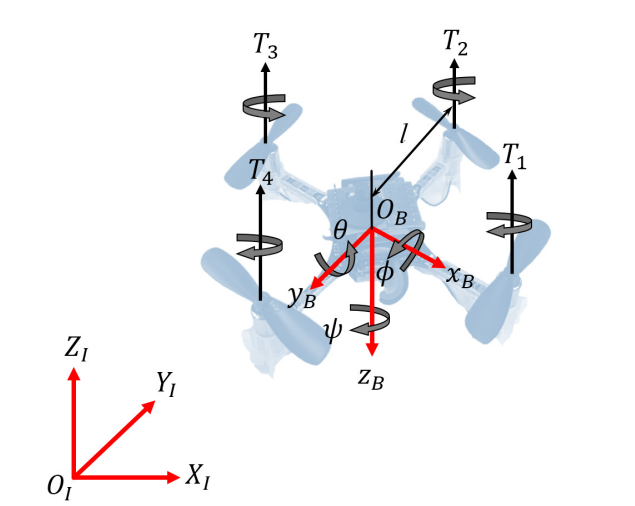
\includegraphics[width=0.55\linewidth]{cuadrupedo_marco_ref.png}
    \caption*{\textit{Nota.} La imagen muestra el sistema de coordenadas inercial y el sistema de coordenadas del cuerpo de un cuadricóptero. Imagen obtenida de \cite{kim2020quadrotorSurvey}.}
    \label{fig:sistema_coordenadas_cuadricoptero}
\end{figure}
\section{Plataforma crazyflie 2.1}
El Crazyflie 2.1 es un mini cuadricóptero versátil y de código abierto desarrollado por la empresa Bitcraze. Esta plataforma tiene un peso aproximado de 29 g y dimensiones de 92×92×29 mm, lo que la hace adecuada para aplicaciones de investigación, educación y pruebas en espacios interiores. La comunicación con el dron se hace por medio de la antena crazyradio 2.0, esta es una antesna de baja latencia.

La arquitectura del Crazyflie 2.1 puede entenderse a partir de dos componentes principales de procesamiento. El primero es el microcontrolador nRF51822, encargado principalmente de la comunicación por radio, Bluetooth de baja energía, lógica de encendido, gestión de batería y detección de placas de expansión. El segundo es el microcontrolador STM32F405, que realiza las tareas principales de control de vuelo, lectura de sensores, telemetría y control de motores.

Una parte importante de esta arquitectura es el \textit{Commander Framework}, encargado de recibir los \textit{setpoints} o referencias deseadas de movimiento. Estos setpoints pueden representar una posición, velocidad u orientación que el dron debe alcanzar. A partir de estas referencias, el sistema de control interno intenta llevar el estado estimado del Crazyflie hacia el estado deseado. \cite{bitcraze_stabilizer_module}

\begin{figure}[H]
    \centering
    \caption{Flujo del módulo estabilizador.}
    \label{fig:flujo_modulo_estabilizador}
    
    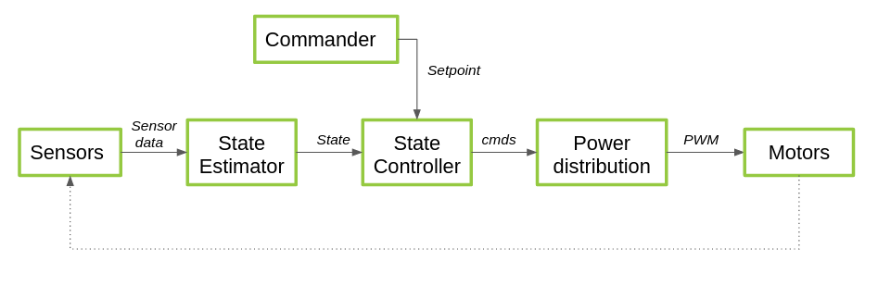
\includegraphics[width=0.75\linewidth]{Commander_framework.png}
    
    \vspace{2mm}
    \begin{flushleft}
        \footnotesize
        \textit{Nota.} La figura muestra el flujo de información desde los sensores hasta los motores dentro del módulo estabilizador del Crazyflie 2.1. Adaptado de Bitcraze \cite{bitcraze_stabilizer_module}.
    \end{flushleft}
\end{figure}
\section{Filtro Kalman y control de Crazyflie 2.1}

El filtro de Kalman es un método matemático utilizado para estimar el estado de un sistema dinámico a partir de información proveniente de un modelo y de mediciones realizadas por sensores. Su utilidad principal es que permite combinar distintas fuentes de información, incluso cuando estas presentan ruido, errores o diferentes frecuencias de actualización. De esta manera, el sistema puede obtener una estimación más confiable que la que se tendría al utilizar únicamente un sensor de forma independiente.\cite{kalman1960}

En el caso del Crazyflie 2.1, el dron cuenta con sensores internos que le permiten estimar su movimiento y estabilidad, como el acelerómetro, el giroscopio y el barómetro. Estos sensores entregan información importante sobre la orientación, aceleración y comportamiento dinámico del dron. Sin embargo, por sí solos no siempre son suficientes para conocer con precisión la posición absoluta del dron dentro de un espacio de trabajo, ya que pueden presentar ruido o acumulación de error durante el vuelo.\cite{schwendener2025desarrollo}

Por esta razón, para lograr un vuelo estable y preciso resulta útil incorporar mediciones externas de posición y orientación. La plataforma Crazyflie permite integrar información proveniente de sistemas del \textit{MoCap}, los cuales permiten conocer la pose del dron dentro del espacio de trabajo. Esta información se introduce al filtro de Kalman extendido, donde se combina con los datos de los sensores internos para mejorar la estimación del estado del dron \cite{bitcraze_state_estimation}.
\begin{figure}[H]
    \centering
    \caption{Entradas y salidas del filtro de Kalman extendido del Crazyflie.}
    \label{fig:ekf_mocap}

    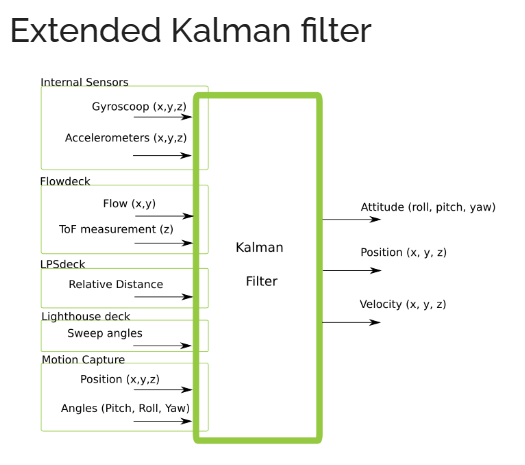
\includegraphics[width=0.78\linewidth]{Extended_Kalman_Filter.png}

    \vspace{2mm}
    \begin{flushleft}
        \footnotesize
        \textit{Nota.} La figura muestra las distintas fuentes de medición que pueden alimentar el filtro de Kalman extendido del Crazyflie. \cite{bitcraze_state_estimation}.
    \end{flushleft}
\end{figure}
\section{Sistemas de captura de movimiento}

Un sistema de captura de movimiento (\textit{Motion Capture}, MoCap) permite registrar la posición y orientación de un objeto dentro de un espacio tridimensional definido. En los sistemas ópticos basados en marcadores, las cámaras registran la luz reflejada o emitida por marcadores colocados sobre el objeto o sujeto de interés. A partir de estas detecciones, el sistema reconstruye la posición tridimensional de los marcadores y permite representar digitalmente su movimiento dentro del volumen de captura .

Existen distintos tipos de marcadores utilizados en sistemas MoCap. Los marcadores pasivos no emiten luz propia, sino que reflejan la luz infrarroja emitida por las cámaras. Por otro lado, los marcadores activos incorporan un emisor de luz, generalmente infrarroja, que permite su detección por parte del sistema. En ambos casos, los marcadores se adhieren al objeto o cuerpo de interés para que el sistema pueda reconstruir su movimiento a partir de sus posiciones en el espacio. \cite{ghorbani2021soma}

Los sistemas ópticos pasivos con marcadores reflectivos y cámaras infrarrojas son ampliamente utilizados debido a que no generan interferencias electromagnéticas y resultan poco intrusivos, ya que únicamente requieren colocar marcadores sobre la superficie del objeto. Sin embargo, presentan limitaciones cuando los marcadores quedan obstruidos de la línea de visión de las cámaras, ya que esto puede provocar pérdida de información o errores en la reconstrucción del movimiento. Además, en sistemas complejos puede ser necesario utilizar una mayor cantidad de cámaras y marcadores, lo cual incrementa el costo y la complejidad de la instalación \cite{schwendener2025desarrollo}.

En el ecosistema Robotat, el sistema MoCap disponible es de tipo pasivo y está conformado por  6 cámaras OptiTrack con un área de trabajo de 400 X 500 X 200 cm. Este sistema permite obtener información de posición absoluta de los objetos dentro del espacio de trabajo con variaciones milimétricas, lo que lo convierte en una herramienta adecuada para aplicaciones de control y seguimiento de trayectorias en interiores \cite{schwendener2025desarrollo}. Para este trabajo, esta característica es especialmente importante, ya que el sistema MoCap puede utilizarse tanto para conocer la posición del Crazyflie 2.1 como para registrar los movimientos del usuario durante la ejecución de gestos.


	\fi
\fi

% CAPÍTULOS
% ----------------------------------------------------------------------------
\newpage
\ifdefined\parpordefecto
	\defaultparformat{j-capitulos}
\else
	\chapter{¿Cómo emplear esta plantilla? (Cuerpo del trabajo)}

El cuerpo del trabajo es la parte sustancial, ya que presenta y examina los datos recopilados durante la investigación. Además, en el caso de modalidad de tesis defiende la hipótesis o tesis, incluso, la puede negar o atacar; por lo tanto, es imperativo que cuente con referencias de fuentes.  

Los capítulos pueden variar según la modalidad de trabajo, por ejemplo: un megaproyecto es diferente a una tesis.

\noindent\rule{\linewidth}{0.4pt}

En el caso particular de este documento, se empleará el cuerpo del trabajo para explicar el uso de la plantilla de \LaTeX como tal. 

\section{¿Cómo trabajar con la plantilla?}

Actualmente se cuenta con dos maneras validadas de trabajar con la plantilla, una \textit{online} (pagada o administrada por la universidad) y una \textit{offline} (gratuita).

\subsection{\textit{Online} mediante Overleaf}

Overleaf (\href{https://www.overleaf.com/}{https://www.overleaf.com/}) es una plataforma que permite trabajar documentos y proyectos de \LaTeX completamente en línea, sin necesidad de instalar ninguna aplicación en el equipo del usuario. Si bien la plataforma deja trabajar documentos de forma gratuita, es necesario contar con una cuenta estudiantil (\$9 al mes) o estándar (\$21 al mes) para trabajar con documentos grandes como la plantilla. Para poder trabajar con esta plantilla en Overleaf siga los siguientes pasos:

\begin{enumerate}
    \itemsep 0em

    \item Abra y habilite / pague una cuenta de estudiante en Overleaf, empleando un correo válido de la universidad.

    \item Cree un nuevo proyecto, seleccionando la opción de Cargar proyecto (Upload project) dentro de las opciones que se le muestran.

    \item Overleaf le dará espacio para cargar un archivo en \texttt{.zip} correspondiente al proyecto. Seleccione el \texttt{.zip} que corresponde a la plantilla y espere a que cargue.

    \item ¡Listo! Ahora podrá editar la plantilla y generar el \texttt{.pdf} de su trabajo de graduación.
    
\end{enumerate}

En su defecto puede solicitar que se le cree su proyecto de trabajo de graduación desde una cuenta profesional de la universidad y se le de acceso como editor. De esta manera podrá obtener las ventajas de la versión pagada desde una cuenta gratis, aunque sólo dentro del proyecto del trabajo de graduación como tal.

Para aprender las generalidades de uso de Overleaf, puede acceder a la documentación en \href{https://es.overleaf.com/learn}{https://es.overleaf.com/learn} o bien acceder a los recursos colocados dentro de la Guía de redacción de trabajos de graduación.

\subsection{\textit{Offline} mediante TeXstudio y MiKTeX}

Una segunda opción para trabajar con la plantilla de manera gratuita, pero \textit{offline}, es mediante la combinación de TeXstudio (\href{https://www.texstudio.org/}{https://www.texstudio.org/}) y MiKTeX (\href{https://miktex.org/}{https://miktex.org/}). Para lograr esto, siga los siguientes pasos:

\begin{enumerate}
    \itemsep 0em

    \item Descargue e instale MiKTeX, asegurando hacerlo con permisos de administrador. Coloque el tamaño de hoja por defecto en \textit{Letter} y que siempre le pregunte/avise antes de instalar paquetes faltantes. Reinicien su equipo para evitar problemas en los siguientes pasos.

    \item Descarguen e instalen TeXstudio, de nuevo asegurando hacerlo con permisos de administrador.

    \item Descomprima el \texttt{.zip} de la plantilla en alguna carpeta de su preferencia, ya que será su directorio de trabajo para el documento. 

    \item Desde el menú de Windows o usando el buscador, abra TeXstudio. 

    \item Dentro de TeXstudio, presione el botón \texttt{Abrir}. Dentro del buscador, ubique la carpeta del paso 3 y seleccione el archivo \texttt{z-main.tex}. 

    \item Vaya a \texttt{Opciones -> Configurar TeXstudio} y luego al menú de Compilar. Asegúrese que el \texttt{Compilador por defecto} sea \texttt{PdfLaTeX} y la \texttt{Herramienta bibliográfica} por defecto sea \texttt{Biber}. Presione \texttt{Aceptar}. 

    \item  Presione el botón de \texttt{Compilar y Ver} (el ``doble play'') y espere, TeXstudio le estará sacando ventanas de diálogo preguntando si desea que instale automáticamente los paquetes que vaya encontrando como faltantes. Ponga atención a cuáles son estos paquetes, por si luego es necesario actualizarlos y/o instalarlos manualmente en caso fallara el instalador automático. 

    \item Luego de esperar el tiempo de compilación deberá tener la pre-visualización del \texttt{.pdf} en el lado derecho, casi idéntico a Overleaf.

    \item En caso no le aparezca el \texttt{.pdf} o le aparezca con errores, actualice los paquetes desde MiKTeX. Para esto, salga de TeXstudio, vaya a \texttt{C: -> Usuarios -> Su nombre de usuario} y borre (en caso aparezca) el archivo \texttt{miktex-console.lock}. Luego corra, desde el menú de Windows o el buscador, la \texttt{MiKTeX Console} y desde ahí vaya a la pestaña de actualizaciones. Indiquen al software que busque actualizaciones y luego que las actualice ahora (cuando se habilite la opción).

    \item Ya cuando haya compilado y visualizado correctamente su documento, puede acceder al \texttt{.pdf} del mismo dentro del directorio de trabajo de su proyecto.
    
\end{enumerate}


\section{¿Cómo utilizar la plantilla?}

Independientemente de la plataforma que se esté empleando para trabajar con la plantilla, en el costado izquierdo podrá encontrar el árbol de navegación para la misma. Dentro de este, podrá identificar archivos con los nombres de las distintas secciones / capítulos del trabajo. Por ejemplo, si presiona el archivo \verb|d-introduccion.tex| encontrará y podrá editar el contenido del capítulo de Introducción. La idea detrás de esto es permitirle al usuario preocuparse únicamente del contenido de las diferentes secciones del trabajo, no del formato. La definición del formato se encuentra dentro del documento \verb|z-main.tex| el cual \textbf{NO DEBE SER MODIFICADO POR EL USUARIO} ya que contiene la definición de la plantilla como tal.

Un documento indispensable a modificar es el de \verb|0-datos_estudiante.tex|. En el mismo se encuentra información tal como el título del trabajo, el autor -- junto con su carrera, carnet y facultad--, el asesor y los miembros de la terna evaluadora (si aplicase), entre otros. Por ejemplo, para cambiar el nombre del autor basta con colocarlo dentro de las llaves de la etiqueta respectiva de la siguiente manera:
\begin{verbatim}
% Datos del estudiante:
% -------------------------------------------------------------------------------
% Nombre completo
\def \nombreestudiante {Nombre Apellido} 
\end{verbatim}

Adicionalmente, este documento permite una personalización básica de la plantilla, como la inclusión de algunas secciones / capítulos opcionales, el formato de referencias bibliográficas y si se quiere o no emplear una imagen de portada distinta al estándar. Se dará más detalle al respecto de esto en una sección posterior.


\section{Figuras, cuadros y ecuaciones}

Una de las grandes ventajas de \LaTeX en comparación a Word o procesadores de documentos similares, es la manera sencilla y automatizada de trabajar con referencias cruzadas. La plantilla busca simplificar aún más este proceso generando automáticamente los índices de figuras y cuadros, al igual que el listado de referencias bibliográficas. Esto siempre y cuando todas estas se definan adecuadamente. 

Para definir figuras, puede emplear la siguiente pieza de código como base:
\begin{verbatim}
\begin{figure}[h] 

    \centering\captionsetup{width=0.8\linewidth}
    \caption{Una imagen de una galaxia.}
    
    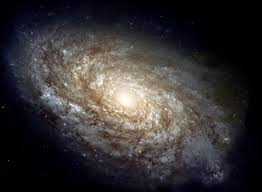
\includegraphics[width=0.5\textwidth]{galaxia.jpg}
    
    \note{La imagen muestra el \textit{render} de una galaxia, generada con 
    base en la información recabada por un telescopio de espacio profundo. 
    Esta imagen fue obtenida de \cite{hoover2010bio}.}
    \label{fig:galaxia}
    
\end{figure}
\end{verbatim}

Esto generará la siguiente figura:
\begin{figure}[h] 
    \centering\captionsetup{width=0.8\linewidth}
    \caption{Una imagen de una galaxia}
    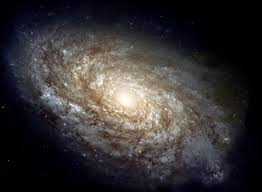
\includegraphics[width=0.5\textwidth]{galaxia.jpg}
    \note{La imagen muestra el \textit{render} de una galaxia, generada con  base en la información recabada por un telescopio de espacio profundo. Esta imagen fue obtenida de \cite{hoover2010bio}.}
    \label{fig:galaxia}   
\end{figure}

\newpage
A detalle
\begin{itemize}
    \itemsep 0em

    \item Las etiquetas \verb|\begin{figure} ... \end{figure}| indican el inicio y final de la figura, estas son parte de la sintaxis estándar de \LaTeX.

    \item La especificación \verb|[h]| dentro de corchetes en \verb|\begin{figure}[h]| indica en dónde deberá colocarse la figura. \verb|[t]| la coloca en la cima de la página, \verb|[b]| en el fondo y \verb|[h]| exactamente en el lugar donde aparece en el texto (esto es lo más similar a la manera en que añaden imágenes en Word). Es importante tomar en consideración que esta especificación es sólo una \textbf{sugerencia} para \LaTeX, ya que este colocará la imagen en donde quede mejor con respecto al espacio disponible. Si quiere forzar a \LaTeX a que respete la especificación, puede añadirle un signo de exclamación al final. Por ejemplo: \verb|\begin{figure}[h!]|.

    \item La etiqueta \verb|\centering| centra la figura y \verb|\captionsetup{width=0.8\linewidth}| indica que el título y la descripción ocuparán sólo el 80\% de los márgenes definidos para el texto. Estas etiquetas corresponden a estándares de formato para la plantilla y \textbf{siempre deberán incluirse tal cual y NO modificarse}.

    \item La etiqueta \verb|\caption{Título}| especifica el título de la figura. Este aparecerá por encima de la misma y alineado hacia la izquierda, y es el que también se ingresará automáticamente al listado. El título debe ser conciso; la descripción más profunda o detalles adicionales deberán colocarse en la Nota, al igual que la referencia bibliográfica si la hubiese. 

    \item \verb|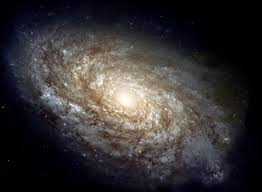
\includegraphics[width=0.5\textwidth]{galaxia.jpg}| hace referencia al archivo como tal de la figura y al tamaño deseado para la misma. En este caso, se está haciendo referencia al archivo de imagen \verb|galaxia.jpg| situado dentro de la carpeta \verb|figuras| en el árbol de navegación. Siempre que las figuras se encuentren dentro de esta carpeta se les podrá referenciar directamente por nombre y extensión de archivo. Con respecto al tamaño, puede establecerse tanto el alto como la altura directamente en unidades (el listado de unidades de tamaño que emplea \LaTeX puede consultarse en la documentación: \href{https://es.overleaf.com/learn/latex/Lengths_in_LaTeX}{https://es.overleaf.com/learn/latex/Lengths\_in\_LaTeX}). En este ejemplo, se está estableciendo el ancho, \verb|width|, como un porcentaje (de 0.0 a 1.0) del tamaño de los márgenes del texto (representado por la etiqueta \verb|\textwidth|). Para una referencia de cómo manejar el tamaño de figuras puede consultar la documentación: \href{https://www.overleaf.com/learn/latex/Questions/How_do_I_specify_the_size_of_an_image_in_LaTeX%3F}{https://www.overleaf.com/learn/latex/Questions/How\_do\_I\_specify\_the\_size\_of\_an\_image\_in\_LaTeX\%3F}.

    \item En caso de requerir una descripción adicional al título o bien brindar más detalles sobre la figura --pero que no se quiera que aparezcan en el índice de figuras--, debe emplearse la etiqueta \verb|\note{...}|. Dentro de esta etiqueta también deberá colocarse la referencia bibliográfica de la figura, si esta se obtuvo de esa manera. En caso que la figura sea de autoría propia deberá colocarse \verb|Elaboración propia.|.

    \item Finalmente, \verb|\label{...}| se emplea para crear una etiqueta que permita a \LaTeX encontrar el recurso cuando se utilicen referencias cruzadas. Todo recurso que quiera referenciarse dentro del texto debe contener una etiqueta y se recomienda emplear alguna convención de nombres para evitar el desorden. Por ejemplo, emplear \verb|\label{fig:nombre_figura}| para figuras, \verb|\label{tab:nombre_cuadro}| para cuadros y \verb|\label{eq:nombre_ecuación}| para ecuaciones. Para referenciar a la figura (o cuadro) dentro del texto se emplea el comando \verb|\ref{etiqueta}|. Por ejemplo, en la Figura \ref{fig:galaxia} puede verse el \textbf{render} de una galaxia, etc. Para el caso de ecuaciones se emplea pero \verb|\eqref{etiqueta}|.

\end{itemize}

Lo anterior se mantiene de la misma manera para cuadros, con la diferencia que deben emplearse las etiquetas \verb|\begin{table} ... \end{table}| para crearlos y deben ``programarse'' acorde a la sintaxis de \LaTeX. La recomendación es no hacer esto manualmente sino más bien emplear alguna herramienta como: 
\begin{itemize}
    \itemsep 0em
    \item \href{https://www.tablesgenerator.com/}{https://www.tablesgenerator.com/}
    \item \href{https://www.latex-tables.com/}{https://www.latex-tables.com/}
    \item \href{https://tableconvert.com/latex-generator}{https://tableconvert.com/latex-generator}
    \item \href{https://www.underleaf.ai/tools/latex-table-generator}{https://www.underleaf.ai/tools/latex-table-generator}
\end{itemize}

Por ejemplo, el Cuadro \ref{tab:experimentos_preliminares}
\begin{table}[h!]
    \centering\captionsetup{width=0.8\linewidth}
    \caption{Resultados del primer set de experimentos.}
    \begin{tabular}{c|ccc}
    \textbf{experimento} & variable 1 & variable 2 & variable 3 \\ \hline
    \textbf{1}           & 12.1       & 1          & 0          \\
    \textbf{2}           & -5.4       & 0          & 25         \\
    \textbf{3}           & 20.2       & 1          & 99        
    \end{tabular}
    \note{Los valores para la variable 2 son binarios mientras que los de la variable 3 son porcentuales. Elaboración propia.} 
    \label{tab:experimentos_preliminares}  
\end{table}

fue creado empleando el siguiente código:
\begin{verbatim}
\begin{table}[h]

    \centering\captionsetup{width=0.8\linewidth}
    \caption{Resultados del primer set de experimentos.}
    
    \begin{tabular}{c|ccc}
    \textbf{experimento} & variable 1 & variable 2 & variable 3 \\ \hline
    \textbf{1}           & 12.1       & 1          & 0          \\
    \textbf{2}           & -5.4       & 0          & 25         \\
    \textbf{3}           & 20.2       & 1          & 99        
    \end{tabular}
    
    \note{Los valores para la variable 2 son binarios mientras que los de 
    la variable 3 son porcentuales. Elaboración propia.}
    \label{tab:experimentos_preliminares}
    
\end{table}
\end{verbatim}

Para ecuaciones deben emplearse las etiquetas \verb|\begin{equation} ... \end{equation}| para crearlas. Dentro de estas la definición de las expresiones se hace mediante el modo matemático de \LaTeX. Si usted tiene experiencia previa con el mismo entonces puede escribir manualmente el código, sino también puede apoyarse de las siguientes herramientas:

\begin{itemize}
    \itemsep 0em

    \item \href{https://latexeditor.lagrida.com/}{https://latexeditor.lagrida.com/}

    \item \href{https://editor.codecogs.com/}{https://editor.codecogs.com/}

    \item \href{https://www.sciweavers.org/free-online-latex-equation-editor}{https://www.sciweavers.org/free-online-latex-equation-editor}

    \item \href{https://www.hostmath.com/}{https://www.hostmath.com/}

    \item En Overleaf puede trabajarse con un editor visual en lugar que el editor de código por defecto. Este editor permite crear ecuaciones de manera similar a Word. Puede ver cómo emplear este tipo de edición en el siguiente video: \href{https://youtu.be/hQ_sC0O-7Wg?si=r5gaTdL6e1LNkXML}{https://youtu.be/hQ\_sC0O-7Wg?si=r5gaTdL6e1LNkXML}.
\end{itemize}

o bien acudir a la documentación: \href{https://es.overleaf.com/learn/latex/Mathematical_expressions}{https://es.overleaf.com/learn/latex/Mathematical\_expressions}. Por ejemplo, la ecuación \eqref{eq:ejemplo_integral}
\begin{equation}
    F(x)=\int_{-\infty}^{x} f(s) ds,
    \label{eq:ejemplo_integral}
\end{equation}

puede generarse mediante el código:
\begin{verbatim}
\begin{equation}
    F(x)=\int_{-\infty}^{x} f(s) ds,
    \label{eq:ejemplo_integral}
\end{equation} 
\end{verbatim}


\section{Numeración y viñetas}

Para crear listados numerados o de viñetas, deben emplearse las etiquetas \newline \verb|\begin{enumerate} ... \end{enumerate}| o \verb|\begin{itemize} ... \end{itemize}| respectivamente. Cada ítem en el listado debe iniciarse con \verb|\item| y puede modularse la separación entre las mismas mediante \verb|\itemsep|. Por ejemplo, el siguiente código:
\begin{verbatim}
\begin{itemize}
    \item Primer elemento.

    \item Segundo elemento.

    \item Tercer elemento.

    \item Etc.
\end{itemize}
\end{verbatim}

produce el listado con viñetas:
\begin{itemize}
    \item Primer elemento.

    \item Segundo elemento.

    \item Tercer elemento.

    \item Etc.
\end{itemize}

Como segundo ejemplo, el código:
\begin{verbatim}
\begin{enumerate}
    \itemsep 0cm 
    
    \item Primer paso.

    \item Segundo paso.

    \item Tercer paso.

    \item Y así sucesivamente.
\end{enumerate}
\end{verbatim}

produce el listado numerado siguiente, en donde se empleó \verb|\itemsep| para eliminar el espacio entre elementos.
\begin{enumerate}
    \itemsep 0cm 
    
    \item Primer paso.

    \item Segundo paso.

    \item Tercer paso.

    \item Y así sucesivamente.
\end{enumerate}

\section{Referencias bibliográficas}

El manejo de referencias bibliográficas dentro de la plantilla se trabaja mediante BibTeX (\href{https://www.overleaf.com/learn/latex/Bibliography_management_with_bibtex}{https://www.overleaf.com/learn/latex/Bibliography\_management\_with\_bibtex}). Este permite crear referencias cruzadas simples a las referencias mediante el comando \verb|\cite{referencia}|, siempre y cuando la referencia se haya definido correctamente dentro del fichero \verb|m-bibliografia.bib|. Si bien puede crearse manualmente cada ficha bibliográfica, como se muestra en el siguiente ejemplo (que aparece dentro del fichero \verb|m-bibliografia.bib|) 

\begin{verbatim}
@article{park2014design,
  title={Design and control of a bio-inspired soft wearable robotic device for 
  ankle--foot rehabilitation},
  author={Park, Yong-Lae and Chen, Bor-rong and P{\'e}rez-Arancibia, N{\'e}stor 
  O and Young, Diana and Stirling, Leia and Wood, Robert J and Goldfield, Eugene 
  C and Nagpal, Radhika},
  journal={Bioinspiration \& biomimetics},
  volume={9},
  number={1},
  pages={016007},
  year={2014},
  publisher={IOP Publishing}
}
\end{verbatim}

se prefiere emplear herramientas que automaticen este proceso, ya que no sólo las fichas individuales son extensas sino que cambian de campos requeridos dependiendo del tipo de fuente. Dos de las herramientas de manejo de referencias estándar en investigación son Mendeley (\href{https://www.mendeley.com/search/}{https://www.mendeley.com/search/}) y Zotero (\href{https://www.zotero.org/}{https://www.zotero.org/}), con las cuales puede generarse el contenido del fichero \texttt{.bib} automáticamente, como se muestra en el siguiente video \href{https://youtu.be/avwPBvaYgw4?si=YBZj3l3QhzO47oDS}{https://youtu.be/avwPBvaYgw4?si=YBZj3l3QhzO47oDS}.
 
\ifdefined\usarAPA
    Para la referencia que se definió anteriormente, basta con emplear \verb|\parencite{park2014design}| para que aparezca dentro del texto de la siguiente manera \parencite{park2014design}.
\else
    Para la referencia que se definió anteriormente, basta con emplear \verb|\cite{park2014design}| para que aparezca dentro del texto de la siguiente manera \cite{park2014design}.
\fi

En caso no tenga experiencia previa empleando Mendeley y/o Zotero, puede consultar los recursos dentro de la guía para la redacción de trabajos de graduación.

\section{Personalización}

La plantilla permite cierto grado de personalización, accesible principalmente a través del resto del archivo \verb|0-datos_estudiante.tex|. Primero, puede emplearse el símbolo \verb|%| para activar y desactivar capítulos, secciones y configuraciones adicionales. Por ejemplo, en caso de querer omitir el capítulo de Prefacio basta con preceder su línea respectiva con el símbolo \verb|%|, es decir, \verb|%\def \CAPprefacio {Prefacio}|. Expandiendo esta funcionalidad, la siguiente configuración

\begin{verbatim}
% Capítulos pre-definidos
% -------------------------------------------------------------------------
% Comentar las líneas de las secciones que desean omitirse, por defecto se 
% se incluyen todas.
\def \CAPprefacio {Prefacio}
\def \CAPantecedentes {Antecedentes}
%\def \CAPanexos {Anexos}
\def \CAPglosario {Glosario}

% Sólo puede activarse UNA de las siguientes tres opciones, dependiendo de 
lo que se requiera (revisar la guía de redacción de trabajos de graduación).
\def \CAPhipotesis {Hipótesis}
%\def \CAPdefinicion {Definición del problema}
%\def \CAPalcance {Alcance}
\end{verbatim}

hace que el trabajo incluya los capítulos de Prefacio, Antecedentes y Glosario pero no el de Anexos. Adicionalmente, entre las tres opciones a emplear para el capítulo de Hipótesis / Definición del problema / Alcance, se selecciona la de Hipótesis.

Puede emplearse un estilo de referencias APA, en lugar del estándar IEEE, activando el atributo \verb|\usarAPA|:
\begin{verbatim}
% Referencias: Puede des-comentar la siguiente línea para utilizar el formato de 
referencias APA
%\def \usarAPA {Usar formato APA}
\end{verbatim}

También puede configurarse para que la plantilla genere la hoja de firmas empleando la información del asesor y los evaluadores --para luego ser firmada en el documento como tal-- o bien que utilice una hoja de firmas definida en un archivo \texttt{.pdf} externo. En caso de emplear la segunda opción debe reemplazarse el archivo \verb|hoja_firmas.pdf| con la hoja de firmas y desactivar el atributo \verb|\GENfirmas|, es decir, la línea correspondiente debe verse como \verb|%\def \GENfirmas {Hoja de firmas}|.

Finalmente, la plantilla permite modificar la imagen en la portada mediante el atributo \verb|\imagenportada|:
\begin{verbatim}
% Portada: Puede cambiarse la imagen en la portada al cambiar el nombre del 
% archivo siguiente. NOTA: la imagen debe tener la suficiente resolución 
(1920x768, o más grande pero con una relación 2.5:1) para cubrir el área 
designada. Por defecto se coloca la imagen del CIT.
\def \imagenportada {plantilla/portadacit-real.png}
\end{verbatim}
Para hacerlo, basta con reemplazar la referencia a la imagen por defecto por la que quiera emplearse (si la coloca dentro de la carpeta de \verb|figuras| sólo deberá colocar el nombre del archivo, sin la referencia a la carpeta). Tome nota que la imagen deberá tener una resolución mínima de \texttt{1920 x 768}, o bien una resolución más grande pero que mantenga una relación de aspecto de \texttt{2.5:1}.

\subsection{Capítulos}

Por la variabilidad que existe entre los trabajos de graduación dependiendo de la modalidad de graduación, carrera y facultad, la plantilla no establece capítulos predeterminados más allá de los obligatorios para todos los casos. Por lo tanto, es responsabilidad del usuario definir los capítulos que necesite dentro del archivo \verb|j-capitulos.tex|. Estos se añadirán automáticamente al índice general junto con las secciones del siguiente nivel de indentación. 

Para definir capítulos adicionales se emplea el comando \verb|\chapter{Nombre del capítulo}|. Pueden definirse --dentro de cualquier capítulo del trabajo-- secciones, sub-secciones y hasta sub sub-secciones, empleando los comandos \verb|\section{...}|, \verb|\subsection{...}| y \\ \verb|\subsubsection{...}| respectivamente. El siguiente código entonces
\begin{verbatim}
\chapter{Ejemplo de capítulo}

\section{Ejemplo de sección}

\subsection{Ejemplo de sub-sección}

\subsubsection{Ejemplo de sub sub-sección}
\end{verbatim}

define un capítulo nuevo con algunas secciones y sub-secciones de prueba

\subsection{Glosario}

El glosario es un capítulo opcional. Se compone de una lista de palabras relacionadas en la investigación, pero desconocidas para el lector. Estas deben presentarse en orden alfabético, junto con su definición. 

Siempre y cuando se encuentre activado, el archivo  \verb|o-glosario.tex| puede emplearse para definir el glosario acorde a la sintaxis de \LaTeX: \href{https://es.overleaf.com/learn/latex/Glossaries}{https://es.overleaf.com/learn/latex/Glossaries}. De esta manera es posible automatizar la generación del glosario y se permitirá el uso de referencias cruzadas para los términos dentro del mismo. 

Por ejemplo, dentro del archivo \verb|o-glosario.tex| se encuentra la definición del término \gls{latex} como
\begin{verbatim}
\newglossaryentry{latex}
{
    name=latex,
    description={Es un lenguaje de marcado adecuado especialmente para la 
    creación de documentos científicos}
}    
\end{verbatim}

Luego de estar definido el término puede emplearse dentro del texto mediante \verb|\gls{latex}|, o bien \verb|\Gls{latex}| si quiere emplearse con mayúscula. Al hacer esto los términos definidos dentro del glosario deberían aparecer de la siguiente forma, por ejemplo, dentro del texto: \gls{formula}, \Gls{latex}.


\chapter{Ejemplo de capítulo}

\section{Ejemplo de sección}
\subsection{Ejemplo de sub-sección}

\subsubsection{Ejemplo de sub sub-sección}

\fi

% CONCLUSIONES
% ----------------------------------------------------------------------------
\ifdefined\CAPconclusiones
	\newpage
	\chapter{Conclusiones}
	\ifdefined\parpordefecto
		\defaultparformat{k-conclusiones}
	\else
		Las conclusiones constituyen otro capítulo. Lo principal es mencionar si se aceptó o rechazó la hipótesis y si se cumplieron los objetivos. Además, se indica cómo contribuye el trabajo a resolver el problema original. Pueden escribirse en forma de párrafo o con viñetas. Para redactarlas, tome en cuenta lo siguiente:  

\begin{itemize}
    \item Son específicas, no generalizadas. 

    \item Se escriben en orden.

    \item Evitan expresiones como «yo pienso», «opino», «desde mi experiencia», etc.; el investigador debe desaparecer, por lo que se redacta en tercera persona.
    
\end{itemize}
	\fi
\fi

% RECOMENDACIONES
% ----------------------------------------------------------------------------
\ifdefined\CAPrecomendaciones
	\newpage
	\chapter{Recomendaciones}
	\ifdefined\parpordefecto
		\defaultparformat{l-recomendaciones}
	\else
		Las recomendaciones son un capítulo opcional. Plantean nuevas líneas de investigación y señalan las debilidades del trabajo, los problemas en la metodología, etc. 

En caso de haber incluido el capítulo de alcance, las recomendaciones deben estar amarradas con el mismo.
	\fi
\fi

% BIBLIOGRAFÍA
% ----------------------------------------------------------------------------
\ifdefined\CAPbibliografia
	\newpage
    \cleardoublepage\phantomsection
    \renewcommand{\bibname}{Referencias}
	\chapter{\bibname}
    \printbibliography[heading=none]
\fi

% ANEXOS
% ----------------------------------------------------------------------------
\ifdefined\CAPanexos
	\newpage
	\chapter{Anexos}
	\ifdefined\parpordefecto
		\defaultparformat{n-anexos}
	\else
		Los anexos constituyen otro capítulo. Con base en el Diccionario de la Lengua Española, se entiende que es un agregado, es decir, aquello importante para entender el contexto del trabajo. Es necesario redactar un párrafo de introducción que describa el contenido de los anexos. No es necesario explicarlos, solo mencionar qué se incluye en este capítulo, por ejemplo:  

\begin{itemize}
    \item[] En estos anexos, se incluye información adicional para entender el contexto del trabajo. La primera parte presenta [...]. Luego, se muestran [...]. Además, se incluye [...]. Por último, se proporciona [...]-

\end{itemize}

Esto guiará al lector, ya que no debe asumirse que sabe lo mismo que el autor, por algo está leyendo el trabajo. Así que sólo copiar y pegar una serie de figuras y cuadros sin un contexto es una falta de cortesía.

Los anexos incluyen material relevante para mayor claridad y profundidad de la investigación, pero distraen al lector si se colocan en el texto del informe. Pueden agregarse cartas, manuales, guías, etc. Es necesario asignar un número a cada anexo de acuerdo con el orden de mención en el desarrollo del trabajo. 

\section{Sección de ejemplo}

Esta corresponde a una sección de ejemplo dentro de los Anexos.
	\fi
\fi

% GLOSARIO
% ----------------------------------------------------------------------------
\ifdefined\CAPglosario
	\newpage
	\printglossary
\fi

\end{document}